
\chapter{\BaFeP Band Character}
\label{Appendix:BandCharacter110Slices}

\begin{figure}[h!]
    \begin{center}
        \includegraphics[scale=0.7]{Chapter3-dHvABaFe2P2/Figures/AngleDepMeasurements/BandCharacterPlot/Band1_110Slice_BandCharacter}
        \caption{Orbital character for band 1 taken across a $[110]$ slice of the Brillouin zone}
        \label{Fig:Appendix:BandCharacter110Band1}
    \end{center}
\end{figure}
%%
\begin{figure}[h!]
    \begin{center}
        \includegraphics[scale=0.7]{Chapter3-dHvABaFe2P2/Figures/AngleDepMeasurements/BandCharacterPlot/Band3_110Slice_BandCharacter}
        \caption{Orbital character for band 3 taken across a $[110]$ slice of the Brillouin zone}
        \label{Fig:Appendix:BandCharacter110Band3}
    \end{center}
\end{figure}
%%
\begin{figure}[h!]
    \begin{center}
        \includegraphics[scale=0.7]{Chapter3-dHvABaFe2P2/Figures/AngleDepMeasurements/BandCharacterPlot/Band4_110Slice_BandCharacter}
        \caption{Orbital character for band 4 taken across a $[110]$ slice of the Brillouin zone}
        \label{Fig:Appendix:BandCharacter110Band4}
    \end{center}
\end{figure}
